\documentclass[11pt]{article}

%\usepackage{fullpage}
%\usepackage{amsfonts}
\usepackage{graphicx}

\def\eq1{y=\frac{x}{3x^2+x+1}}
\def\labellaxes{Rember to include a scale and label your axes}

\begin{document}

\begin{center}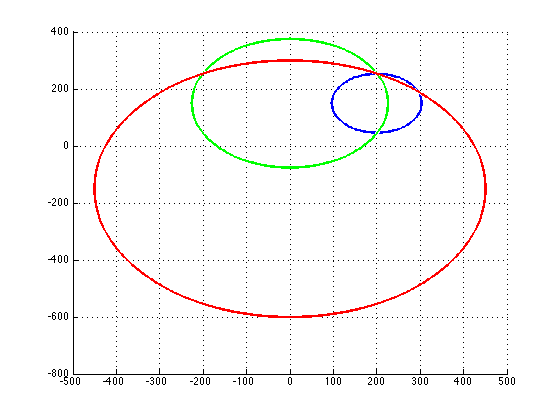
\includegraphics{p2.png}
\end{center}

%    The set of natual number is denoted by $\mathbb{N}$
%    
%     The set of real number is denoted by $\mathbb{R}$
%    
%     The set of Intergers is denoted by $\mathbb{Z}$
     
     Graph $\eq1$. \labellaxes

     
     Identify the asymtotes for the graph of $\eq1$
     
     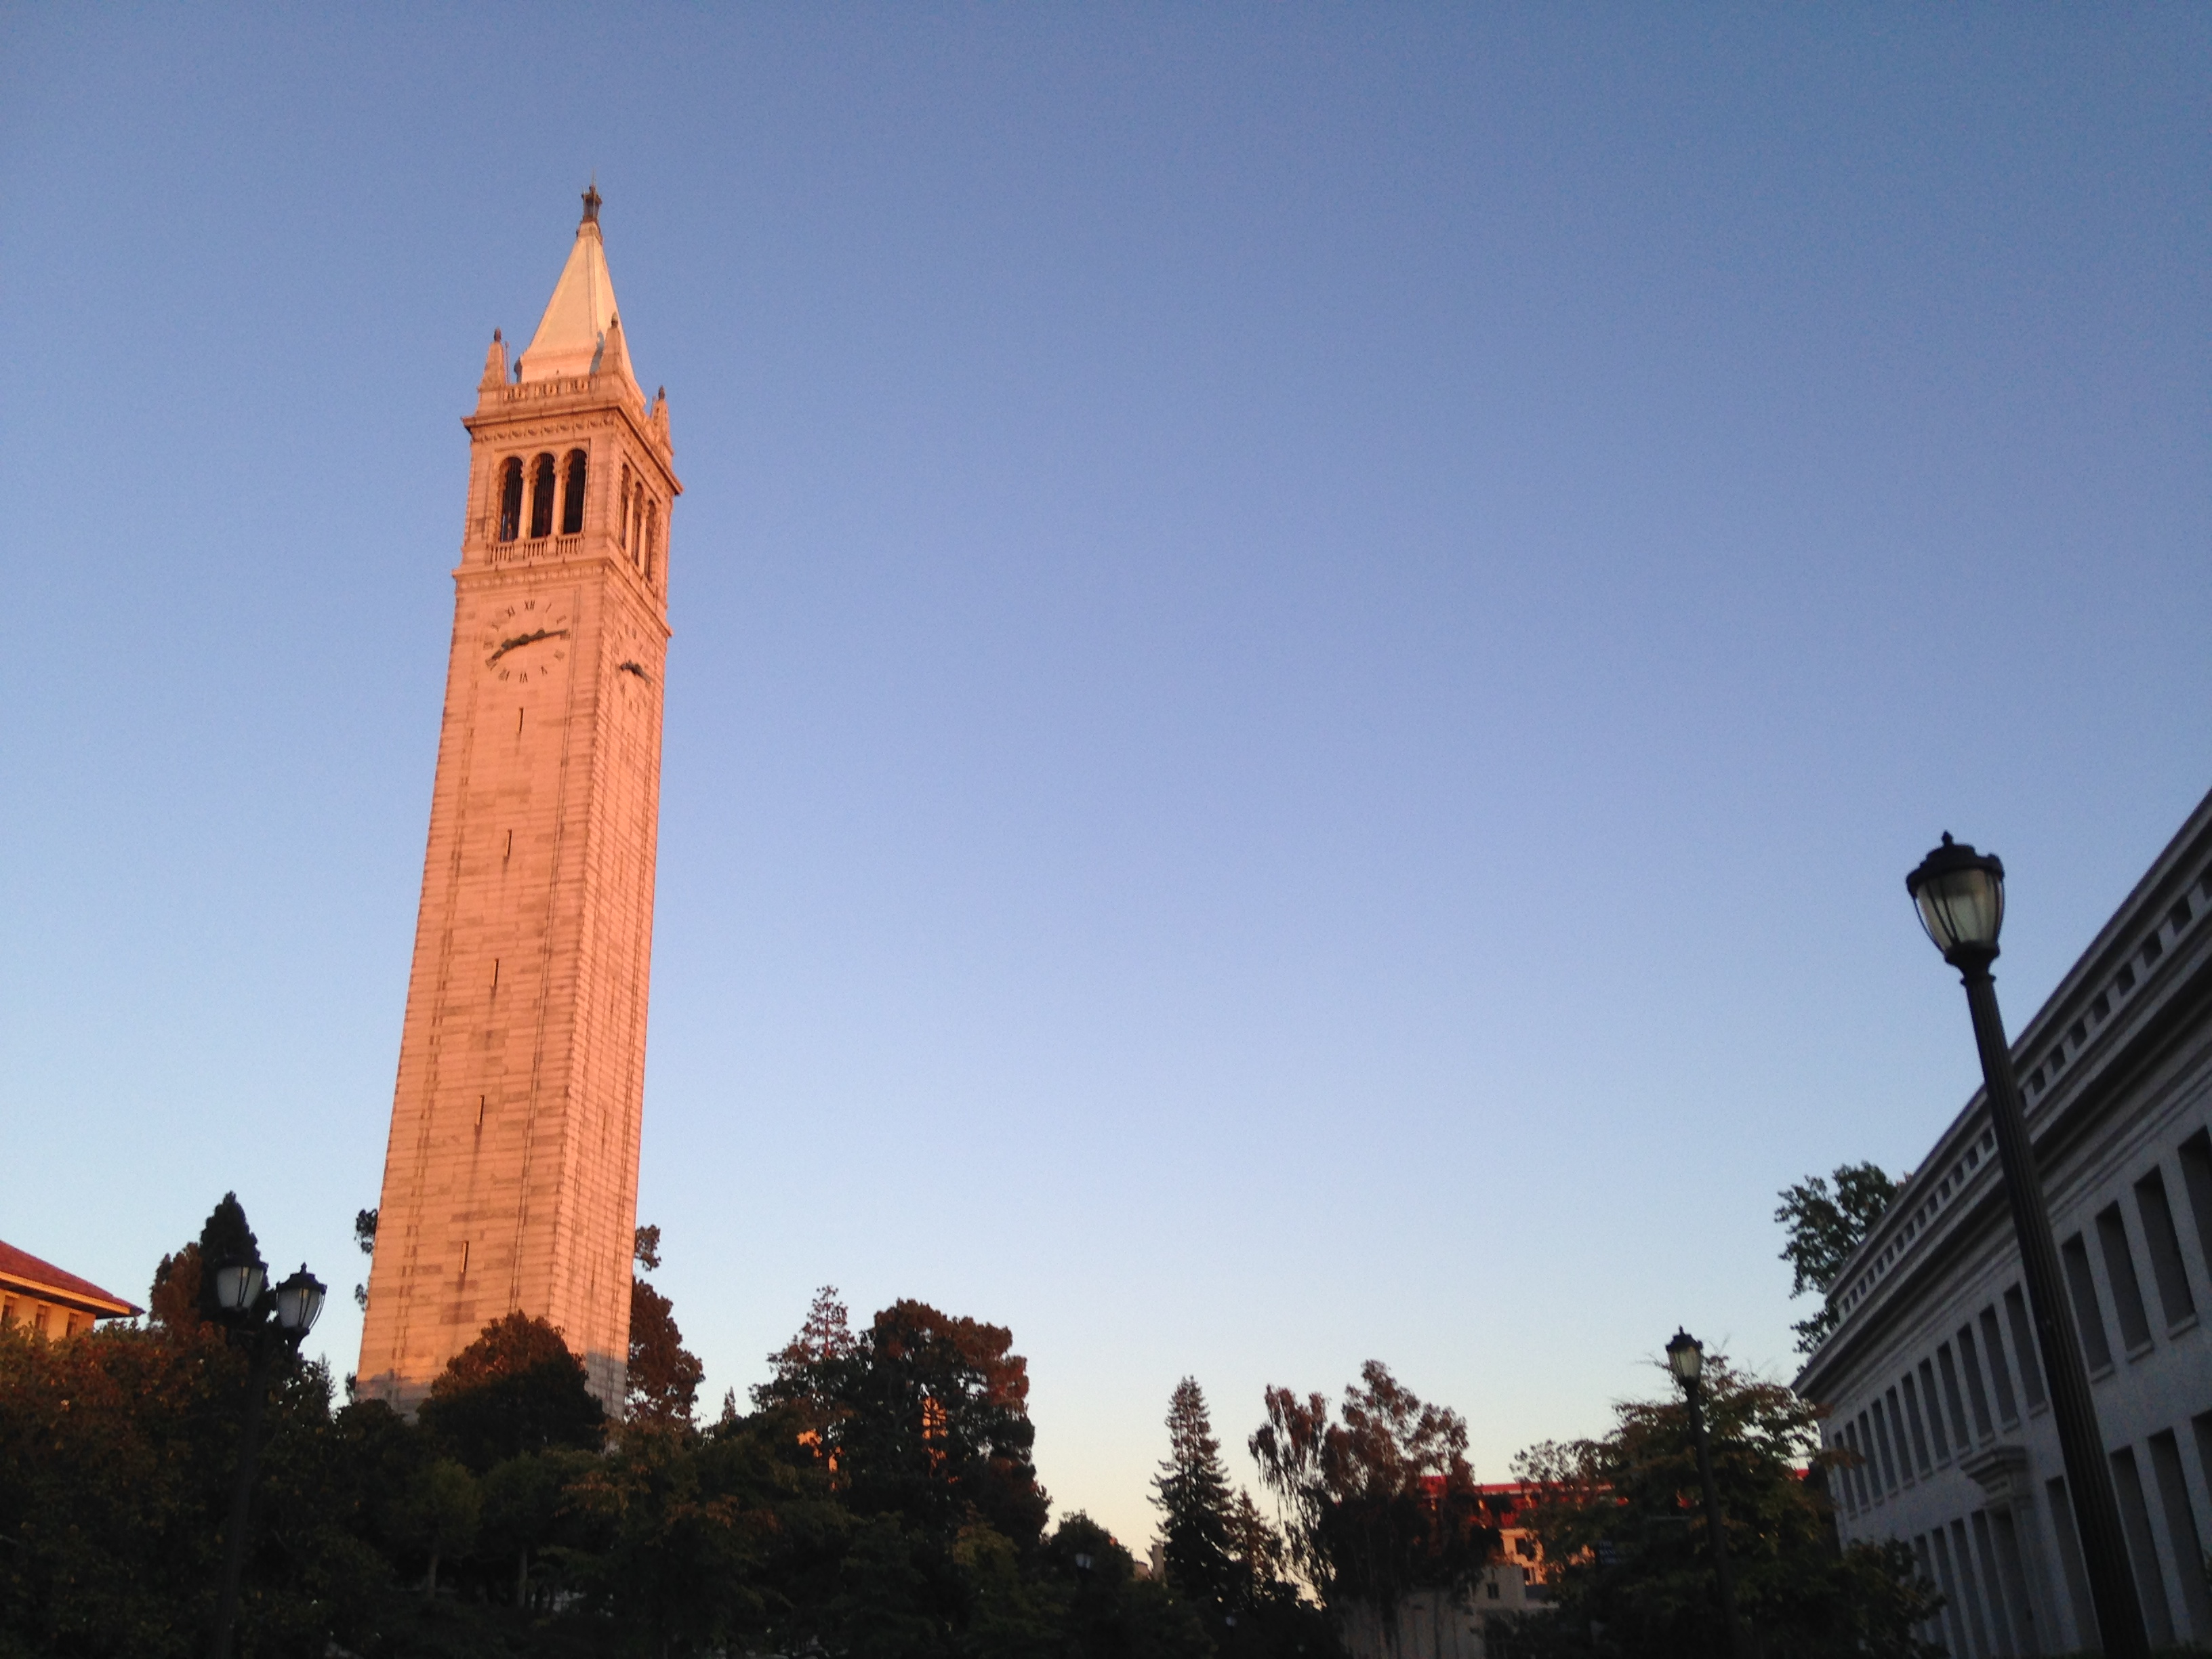
\includegraphics[width=5in]{IMG_0504}
    
    
\end{document}
